\section{Loss functions}

Since there are two \glspl*{nn}, two loss functions were obtained with the training. They are shown in the~\cref{fig:test_loss}.

\begin{figure}[!htb]
    \centering
    \caption[Loss function versus number of epochs for the neural networks]{Loss function versus number of epochs for the neural networks. The number of epochs in the figure does not represent the total number of epochs in the training.}
    %
    \begin{subfigure}{0.49\textwidth}
        \centering
        \caption{Loss function for NN 1}
        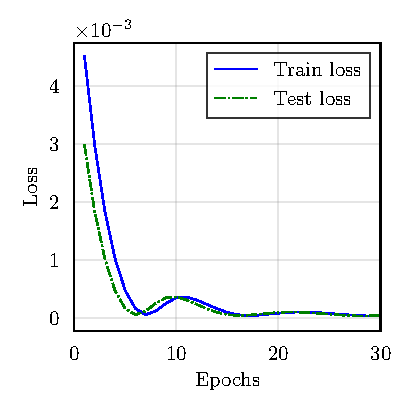
\includegraphics{figures/4results/uav/loss_function_nn1.pdf}
        \label{fig:test_loss_nn1}
    \end{subfigure}
    \hfill
    \begin{subfigure}{0.49\textwidth}
        \centering
        \caption{Loss function for NN 2}
        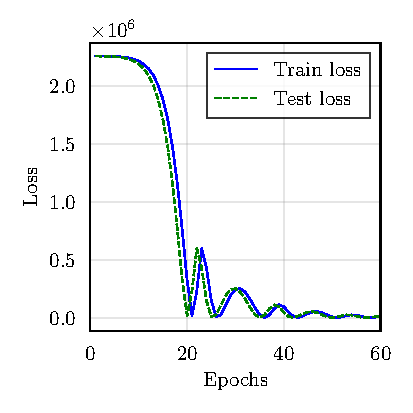
\includegraphics{figures/4results/uav/loss_function_nn2.pdf}
        \label{fig:test_loss_nn2}
    \end{subfigure}

    {\footnotesize Source: prepared by the author.}
    \label{fig:test_loss}
\end{figure}

\section{UAV Forces}

The control forces are generated to make the \gls*{uav} travel in a circular trajectory. From \citet{geronel2023} script, the correspondent trajectory for all the input and output data generated is shown in the~\cref{fig:trajectory}. 
This trajectory is arbitrary chosen and the other ones generated are very similar with noised added.


The normalized forces from neural network \gls*{nn} 1 go through a detailed comparison with the white box script within the corresponding state space. 
This analysis is crucial because it reveals the consistancy of the model, aiming to show insights into the accuracy of \gls*{nn} 1 predictions.
The results are presented in~\cref{fig:forces_normalized}.
The denormalized forces obtained by joining the results of both \gls*{nn} are also presented in~\cref{fig:forces_denormalized}, with the same goal.

\begin{figure}[!htb]
    \centering
    \caption[Trajectory of the UAV]{Trajectory of the UAV. Circular trajectory was chosen and the thousand other ones generated are only variations with noise added.}
    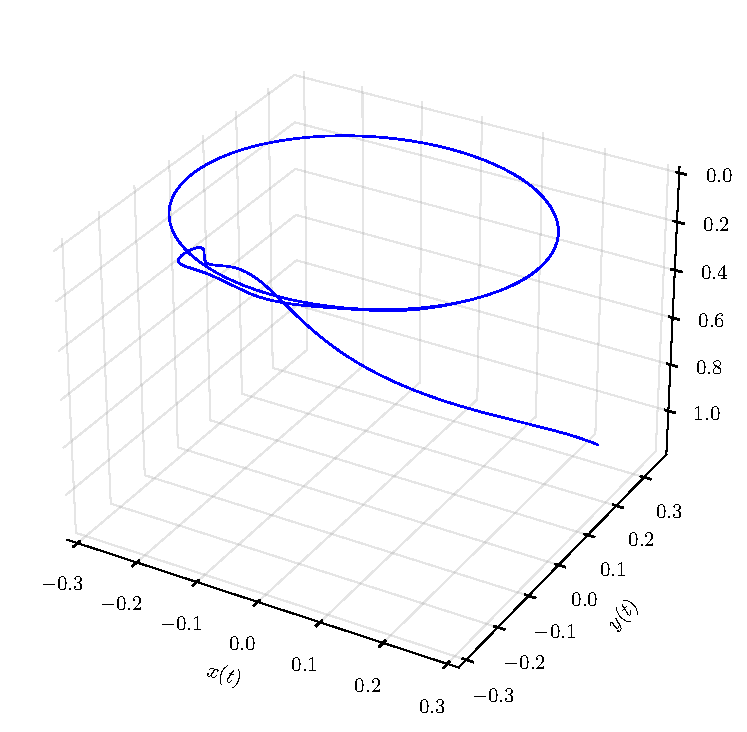
\includegraphics{figures/4results/uav/trajectory.pdf}
    
    {\footnotesize Source: adapted from \citet{geronel2023}}
    \label{fig:trajectory}
\end{figure}

\begin{figure}[!htb]
    \centering
    \caption[Forces normalized obtained from the neural network 1]{Forces normalized obtained from the neural network 1. Comparison is made from the results predicted from the neural network and the normalized preprocessing data, both for input and output data.}
    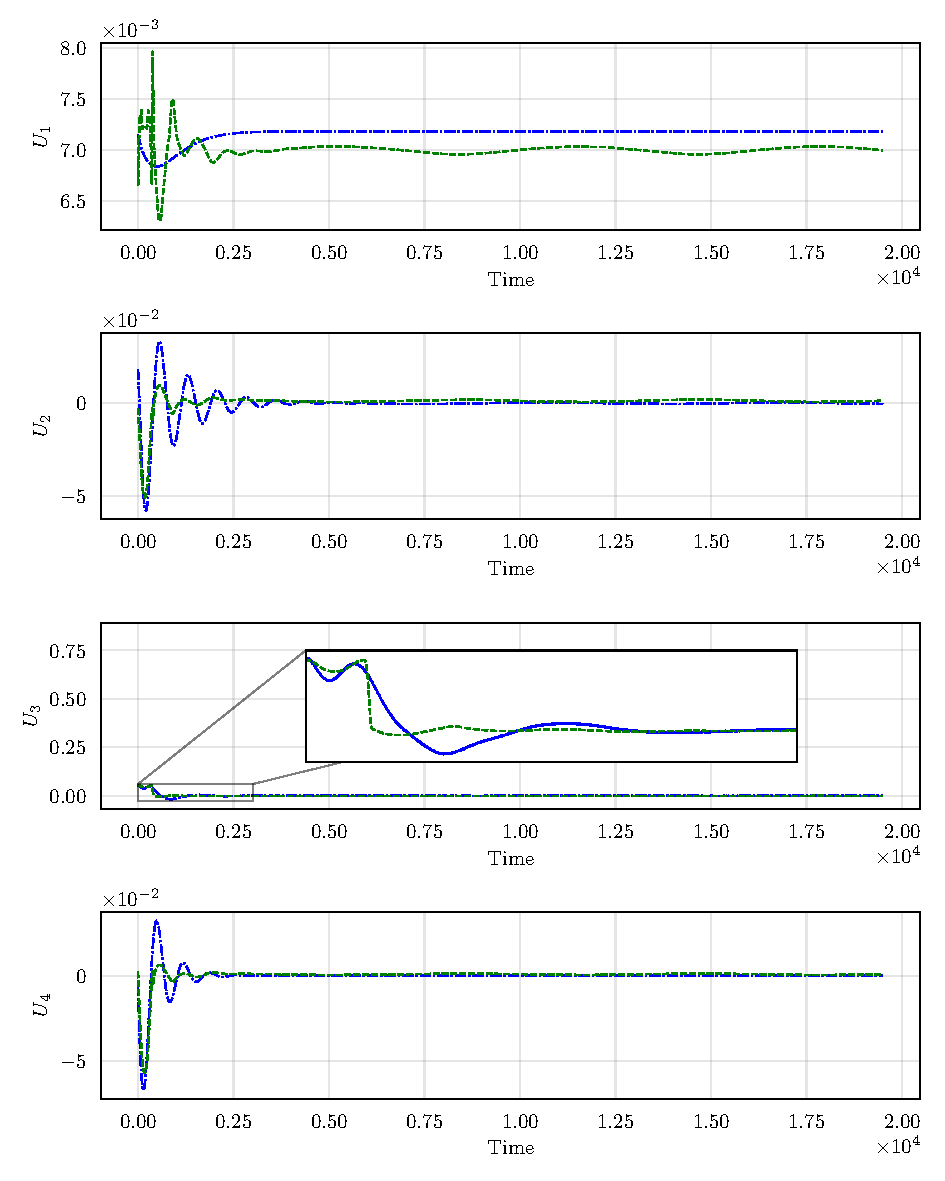
\includegraphics{figures/4results/uav/forces_normalized.pdf}

    {\footnotesize Source: prepared by the author.}
    \label{fig:forces_normalized}
\end{figure}

\begin{figure}[!htb]
    \centering
    \caption[Forces denormalized obtained from the combination of neural network 1 and 2]{Forces denormalized obtained from the combination of neural network 1 and 2. Comparison is made from the results predicted from the combination of both neural network and the raw data got from the white box parametric model.}
    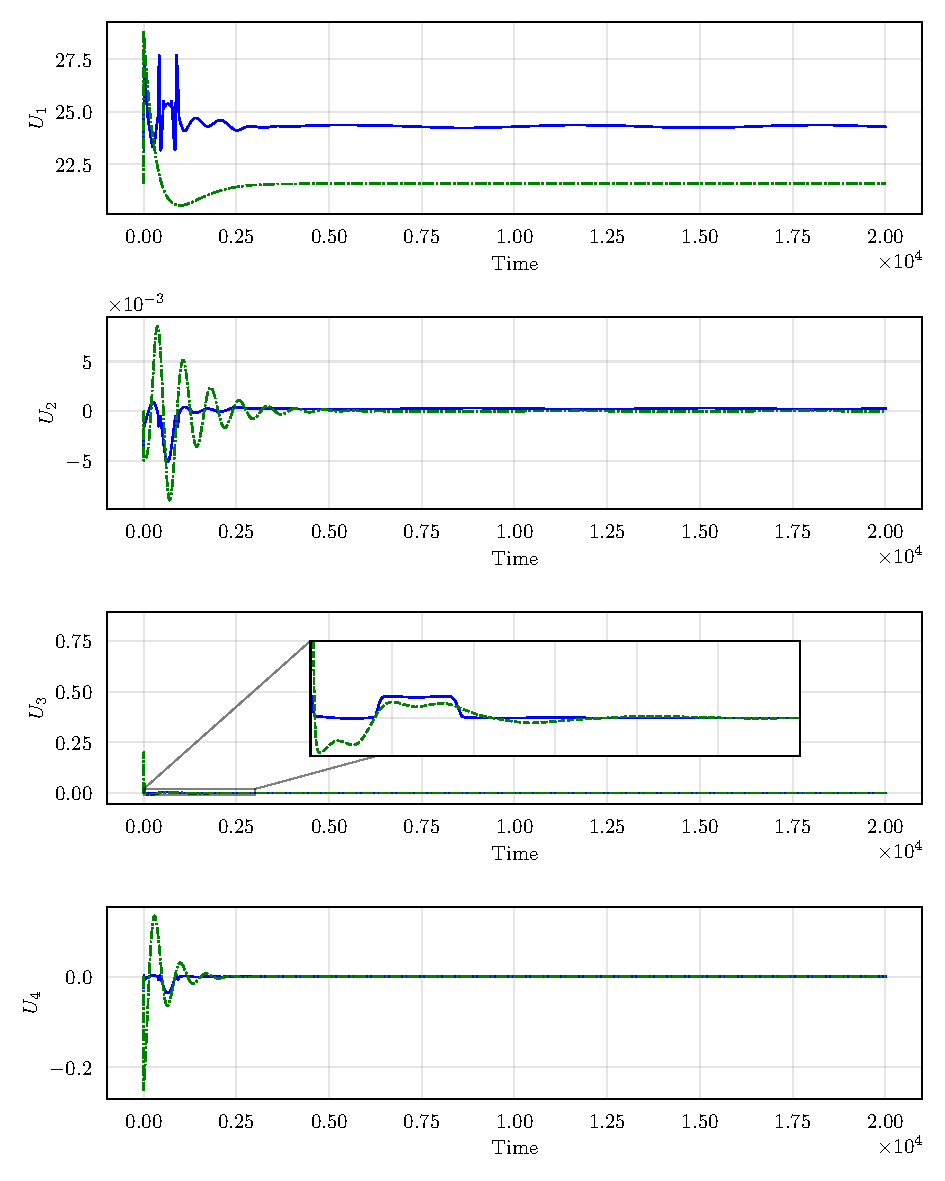
\includegraphics{figures/4results/uav/forces_denormalized.pdf}

    {\footnotesize Source: prepared by the author.}
    \label{fig:forces_denormalized}
\end{figure}



